% !Tex root = main.tex
\newpage
\section{Discussion}
\subsection{Robustness}
Robustness is introduced in order to measure the imputation-capabilities of an FD using FD Imputer.
It is successfully demonstrated that FDs with a high robustness also contain humanly explainable meanings, for example when discussing figure~\ref{fig:f1_fd_adult}.

However, it was possible to demonstrate that FDs do not offer any insights about the profile of data.
They are fit for the specific task of schema normalization.
However, the notion that ``any dependency [could] be turned into a rule to check for errors in the data''~\cite[p.~9]{ABE19} does not seem to be true in general, but only for highly robust FDs with classifiable values in the RHS.

If an FD contains continuous values in the RHS, FD Imputer generally performs poorly.
As shown in table~\ref{tab:fd-imputer-mse}, FD Imputer does not retrieve imputations for most RHSs in the test-set.
In future works, implementing FD Imputer with a selection of RFDs might lead to further insights regarding robustness of dependencies containing continuous RHS values.

\subsection{Comparing ML Imputer with FD Imputer}
FD Imputer is implemented to probe the feasibility of value imputation using FDs.
The usage of FDs for value implementation also makes a comparison with learned classifiers and regression-models possible.

The behavior of FD Imputer is similar to what can be observed when analyzing a case of overfitting.~\cite[p.~56]{SMO08}
Haykins writes that ``[Overfitting] is essentially a `look-up table', which implies that the input-output mapping [\dots] is not smooth.''~\cite[p.~165]{HAY08}
The way FD Imputer functions is \emph{literally} by using the test-set as a look-up table.

\subsubsection{Imputing Sequential RHSs}
Since FDs are established by exact equality of values, imputations of continuous values are very rare and, if they exist, either extremely accurate or very wrong (see table~\ref{tab:fd-imputer-mse-abalone}.
FD Imputer cannot approximate numerical values, due to the definition of an FD.
Data is always assumed to be classifiable.

In contrast to this, ML-Imputer is able to perform regression, predicting a continuous label for a given input with a specific uncertainty.
This circumstance leads to a far superior performance of ML Imputer when imputing continuous values.
Although MSEs for the FD Imputer model are generally smaller than MSEs measured for models trained with DepDetector, this effect is just a manifestation of the overfitting that takes place when FD Imputer looks up values.
This result is emphasized by the findings in table~\ref{tab:fd-imputer-mse}:
On the datasets considered in this work, FD Imputer cannot retrieve imputations from the test-set for an average of 99.8\% of RHS values.

\subsubsection{Imputing Classifiable RHSs}
Figure~\ref{fig:f1_ml_fd_adult} compares the F1-Scores of both ML Imputer and FD Imputer on the Adult dataset.
One can observe that for almost all FDs, ML Imputer performs better than the FD Imputer.
FD Imputer performance and ML Imputer performance appear to be partially proportional.
If the score achieved by ML Imputer is lower than 0.7, the FD Imputer's F1-Score for the same FD is 0.
\begin{figure}[ht]
     \centering
     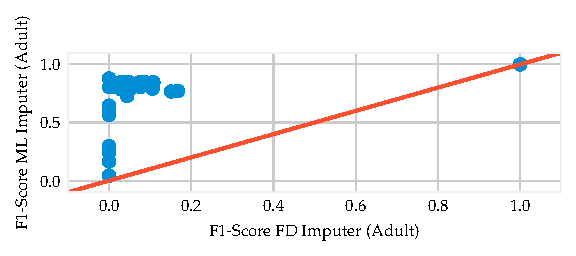
\includegraphics[width=\textwidth]{../figures/adult/f1_ml_fd}
     \caption{The figure compares the F1-Score of the FD Imputer compared to the F1-Score of ML Imputer. Each point represents one FD.}
     \label{fig:f1_ml_fd_adult}
 \end{figure}

However, for FDs where ML Imputer's scores are greater than 0.7, the FD Imputer's scores are greater than 0.
The two FDs for which the FD Imputer performs as well as the ML Imputer were identified and discussed in the previous sections.

\subsubsection{Overfitting ML Imputer}
In order to mimic the overfitting that takes place when FD Imputer looks up imputations on the train-set, it might be interesting to overfit ML Imputer models on purpose.
As shown in figure~\ref{fig:f1-ml-overfit-adult} and figure~\ref{fig:mse-ml-overfit-fractions}, neither the classifier-models, nor the regression-models trained by ML Imputer are capable of overfitting.
Future research-effort could be put into overfitting the models trained by ML Imputer with the goal of approximating the properties of FD Imputer.

\subsection{Dependency Detection with DepDetector}
The DepDetector algorithm was implemented to demonstrate dependency detection using models trained with ERM-strategies.
The `greedy' search-strategy was successfully used to detect minimal dependencies that are robust towards noise when used for training new models.
The dependencies detected this way are a blend of RFDs as discussed in the theory-section of this work.

Dependencies found with DepDetector can be used to save computation time when training a network for imputation.
Since minimal dependencies are often a subset of the whole relational instance, future imputation tasks can thus be performed more quickly by training models with less data.

Furthermore, minimal dependency detection helps explain the way a trained imputation-model works internally.
By reducing the amount of columns with which a model is trained, the way imputations are derived can often be reconstructed by inspecting the remaining columns.

It was not possible to derive FDs using ERM-strategies.
As discussed in the previous paragraphs, the behavior of FD Imputer might be approximated by overfitting models generated by ML Imputer.
In a future effort to derive robust FDs with DepDetector, it might be suitable to run the DepDetector-algorithm training overfitted models on purpose.

Computing results, especially using the `complete'-strategy, is computationally expensive.
Compared with FD detection algorithms, DepDetector is several orders of magnitude slower when detecting minimal dependencies.
For the Chess-dataset, the `complete'-strategy takes about \( 10^5 \) times longer until it converges, the `greedy'-strategy takes approximately \( 10^4 \) times longer.

DepDetector was implemented as a proof of concept.
There is a big margin for performance improvement.
Better performance can be achieved by training models on GPUs instead of CPUs.
Leveraging asynchronous programming techniques, models on the same level of the search lattice can be trained in parallel.
Furthermore, DepDetector internally models the search lattice as a tree rather than a lattice as in figure~\ref{fig:dep-detector-search-tree}.
This leads to redundant model training.

In general, the DepDetector approach is different from classical FD discovery algorithms in that minimal dependencies are detected solving an optimization problem on a graph.
The score of a parent-node has direct implications for the performance of its child-nodes.
Future research might investigate if this property is advantageous when searching for dependencies on big datasets.

\section{Conclusion}
In pursuit of identifying robust FDs, it is shown that FD Imputer can be used to measure robustness as defined in this work.
Experiments with FD Imputer lead to the conclusion that only FDs with RHSs containing classifiable data can be robust.
Generally, FDs are highly susceptible to noise in data.

A comparison between ML Imputer and FD Imputer suggests that imputation results yielded using FD Imputer are similar to using an overfitted model.
It is not possible to use FDs to impute continuous numerical data.

Dependencies with learned relaxation on the attribute comparison were successfully detected on datasets using machine learning techniques with an algorithm called DepDetector.
Two search-strategies were implemented and benchmarked on eight datasets.
